\documentclass[11pt,a4paper]{article}

\usepackage[utf8]{inputenc}
\usepackage[T1]{fontenc}
\usepackage[french]{babel}
\usepackage{lmodern}
\usepackage{microtype}
\usepackage[margin=2.3cm]{geometry}
\usepackage{booktabs}
\usepackage{tabularx}
\usepackage{array}
\usepackage{xcolor}
\usepackage{enumitem}
\usepackage{float}
\usepackage{graphicx}
\usepackage{amsmath}
\usepackage{pifont}
\usepackage[round,authoryear]{natbib}
\usepackage[colorlinks=true,linkcolor=teal!70!black,citecolor=teal!70!black,urlcolor=teal!70!black]{hyperref}

\newcolumntype{Y}{>{\raggedright\arraybackslash}X}
\newcolumntype{C}[1]{>{\centering\arraybackslash}p{#1}}
\newcommand{\oui}{\textcolor{teal!70!black}{\ding{51}}}
\newcommand{\non}{\textcolor{red!60!black}{\ding{55}}}
\newcommand{\partiel}{\textcolor{orange!80!black}{$\sim$}}
\setlist{itemsep=2pt,topsep=4pt}

\title{\textbf{Router par la preuve et s'abstenir à temps :\\ allocation adaptative du calcul et de la
recherche documentaire pour des LLM locaux}\\[6pt]
\large Une évaluation pré-enregistrée de la qualité, de la latence et de l'énergie sur matériel local}
\author{Alae Lahbichi -- Étudiant en 5\textsuperscript{e} année IA/Data\\[2pt]
\small\href{mailto:a.lahbichi2004@gmail.com}{\texttt{a.lahbichi2004@gmail.com}}\\
\small Code et données : \href{https://github.com/AlaeLahbichi/Adaptive-Compute-and-RAG-for-Efficient-Reliable-Local-LLMs}{\footnotesize\texttt{github.com/AlaeLahbichi/Adaptive-Compute-and-RAG-for-Efficient-Reliable-Local-LLMs}}}
\date{18 octobre 2026}

\begin{document}
\maketitle

\begin{abstract}
\noindent Un système de questions-réponses exécuté sur une machine personnelle doit décider, pour
chaque question, quel modèle de langage utiliser, combien de documents récupérer, et s'il vaut mieux
s'abstenir. Ces trois décisions sont presque toujours étudiées séparément, et leur coût exprimé en prix
d'API plutôt qu'en latence ou en énergie mesurées. Nous proposons une politique adaptative simple qui
les prend conjointement à partir de deux signaux peu coûteux : la \emph{suffisance des preuves},
calculée à partir du score BM25 du meilleur passage, et la \emph{confiance} du modèle, lue dans les
probabilités des tokens générés. Nous l'évaluons sur un Apple M3 Pro avec deux modèles Qwen quantifiés
en 4 bits (1,5 et 4 milliards de paramètres), sur un benchmark de 630 questions dérivé de SQuAD 2.0 et
HotpotQA, avec des critères de succès fixés avant les expériences et un jeu de test utilisé une seule
fois. Sur 450 questions de test, la politique atteint la qualité de la référence « grand modèle + RAG »
(score 0,550 contre 0,537 ; non-infériorité démontrée), avec moins de réponses fausses (risque 0,40
contre 0,42), et dépasse deux routeurs de la littérature fondés sur la question seule (0,489 et 0,517).
Elle ne réduit toutefois la latence que de 10~\% et l'énergie de 9~\%, au lieu des 20~\% visés :
\textbf{le critère principal n'est pas atteint}. L'analyse attribue cet échec au réglage d'un seuil
d'abstention absolu sur un trop petit jeu de développement. Nous détaillons les points faibles de
l'étude et un programme d'améliorations concret.

\medskip
\noindent\textbf{Mots-clés :} LLM locaux, routage de modèles, RAG adaptatif, abstention, efficacité
énergétique, évaluation pré-enregistrée.
\end{abstract}

%======================================================================
\section{Introduction}\label{sec:intro}
%======================================================================

Les modèles de langage (LLM) de quelques milliards de paramètres, quantifiés, tournent désormais sur un
ordinateur portable. Les exécuter localement protège les données et supprime la dépendance à un service
distant, mais chaque requête a un coût direct : temps d'attente, mémoire, énergie. La génération
augmentée par récupération (RAG) améliore la factualité \citep{gao2023ragsurvey}, mais elle allonge le
prompt et donc la latence. Un grand modèle répond mieux qu'un petit, mais plus lentement. Et lorsque
les documents ne contiennent pas la réponse, le meilleur choix est souvent de ne pas répondre
\citep{wen2024abstention}.

Appliquer la configuration la plus coûteuse à toutes les questions gaspille des ressources sur les
questions faciles ; appliquer la moins coûteuse dégrade la qualité sur les questions difficiles. D'où la
question de recherche :

\begin{quote}
\emph{Comment allouer automatiquement, et de manière mesurable, les ressources de calcul et de recherche
documentaire à chaque requête, afin de réduire le coût d'un système LLM local sans dégrader
significativement la qualité, la factualité et la fiabilité des réponses ?}
\end{quote}

Elle se décline en quatre questions :
\begin{description}[style=sameline,leftmargin=1.2cm]
\item[QR1] Un signal peu coûteux permet-il de choisir le modèle et le niveau de recherche sans perte de qualité ?
\item[QR2] Peut-on décider de l'abstention de manière fiable, en combinant incertitude du modèle et qualité des preuves ?
\item[QR3] Quel compromis qualité--latence--énergie obtient-on sur matériel local, une fois le coût des signaux compté ?
\item[QR4] Les gains sont-ils homogènes selon le type de question ?
\end{description}

\paragraph{Contributions.}
\begin{enumerate}
\item Une revue de littérature qui montre que le choix du modèle, la décision de recherche et
l'abstention sont étudiés séparément, avec un coût rarement mesuré en local (section~\ref{sec:etat}).
\item Un \textbf{benchmark et un protocole pré-enregistrés} sur matériel local : critères de succès
écrits avant les expériences, jeu de test utilisé une seule fois, latence mesurée sur trois passes,
énergie mesurée par \texttt{powermetrics} (sections~\ref{sec:protocole} et~\ref{sec:pilote}).
\item Des \textbf{méthodes de référence} : six stratégies fixes et deux routeurs inspirés de RouteLLM et
d'Adaptive-RAG (section~\ref{sec:references}).
\item Une \textbf{politique adaptative conjointe} (modèle $\times$ nombre de passages $\times$ abstention),
fondée sur deux signaux quasi gratuits et interprétables (section~\ref{sec:politique}).
\item Une \textbf{évaluation finale} honnête, qui aboutit à un résultat partiellement négatif, et un
\textbf{programme d'améliorations} fondé sur l'analyse de ses causes
(sections~\ref{sec:final} à~\ref{sec:faiblesses}).
\end{enumerate}

%======================================================================
\section{État de l'art}\label{sec:etat}
%======================================================================

\paragraph{Méthode de revue.} Les sources consultées sont arXiv, ACL Anthology, OpenReview, Google
Scholar, Semantic Scholar et les actes de NeurIPS, ICLR, AAAI et MLSys. Les requêtes combinent
\textit{LLM routing}, \textit{model cascade}, \textit{adaptive retrieval}, \textit{adaptive RAG},
\textit{uncertainty estimation}, \textit{selective prediction}, \textit{abstention} et
\textit{energy-aware LLM inference}. Sont retenus les travaux qui adaptent, requête par requête, le
choix du modèle, la recherche ou la décision de répondre, avec une évaluation expérimentale, ainsi que
les mesures de coût d'inférence et les jeux de données utiles. Sur 51 références identifiées (recherche
initiale, \emph{snowballing} et recherche croisée sur arXiv), 46 ont été retenues et classées par thème.

\subsection{Routage et cascades de modèles}

\emph{Router}, c'est choisir avant la génération le modèle qui traitera une requête ; une
\emph{cascade} interroge d'abord un modèle peu coûteux et n'escalade vers un plus puissant que si sa
réponse semble peu fiable. FrugalGPT \citep{chen2023frugalgpt} enchaîne des modèles de coût croissant et
s'arrête dès qu'un scoreur appris juge la réponse fiable. AutoMix \citep{aggarwal2023automix} escalade
selon une auto-vérification, et \citet{yue2023cascades} selon la cohérence entre réponses. Hybrid LLM
\citep{ding2024hybrid} prédit la difficulté de la requête pour envoyer les plus simples au petit modèle ;
RouteLLM \citep{ong2024routellm} apprend des routeurs fort/faible à partir de préférences humaines.
D'autres approches utilisent un bandit manchot \citep{nguyen2024metallm} ou un modèle de récompense
\citep{lu2023zooter}. RouterBench \citep{hu2024routerbench} propose un cadre d'évaluation commun, et la
revue de \citet{varangot2025survey} constate que le coût y est presque toujours un prix d'API. Plus
récemment, \citet{fu2026inflation} utilisent un signal local avant exécution et un coût réel en tokens,
et RACER \citep{hao2026racer} apporte des garanties conformes, c'est-à-dire valides sans hypothèse sur la
distribution des données.

\subsection{RAG adaptatif}

\citet{mallen2022trust} montrent que la recherche est surtout utile pour les connaissances rares, et
peut nuire pour les connaissances courantes. Adaptive-RAG \citep{jeong2024adaptiverag} entraîne un
classifieur de complexité qui choisit entre aucune, une ou plusieurs étapes de recherche. FLARE
\citep{jiang2023flare} et DRAGIN \citep{su2024dragin} déclenchent la recherche pendant la génération
lorsque le modèle devient incertain. Self-RAG \citep{asai2023selfrag} apprend au modèle à juger
lui-même la pertinence des passages ; Corrective RAG \citep{yan2024crag} évalue la qualité des documents
et les corrige ou les filtre ; Tiny-Critic RAG \citep{wu2026tinycritic} confie ce jugement à un petit
modèle. \citet{moskvoretskii2025adaptive} comparent 27 méthodes et montrent que des signaux
d'incertitude simples rivalisent avec des pipelines complexes. RAGRouter-Bench
\citep{wang2026ragrouterbench} et Self-Routing RAG \citep{wu2025srrag} routent entre paradigmes de RAG,
et LeanContext \citep{arefeen2024leancontext} réduit le contexte récupéré pour en diminuer le coût.

\subsection{Incertitude et abstention}

Les probabilités internes des grands modèles sont raisonnablement calibrées \citep{kadavath2022know}.
L'entropie sémantique \citep{kuhn2023semantic} et SelfCheckGPT \citep{manakul2023selfcheckgpt} exploitent
la cohérence entre plusieurs réponses échantillonnées, au prix de plusieurs générations ; la confiance
exprimée en mots n'est fiable qu'après un apprentissage dédié \citep{lin2022verbal}.
\citet{kamath2020selective} formalisent la réponse sélective et ses deux mesures : la \emph{couverture}
(part des questions auxquelles le système répond) et le \emph{risque} (part d'erreurs parmi ces
réponses). La revue de \citet{wen2024abstention} montre que l'abstention reste rarement intégrée aux
systèmes de RAG.

\subsection{Coût et énergie de l'inférence}

\citet{samsi2023watts} mesurent l'énergie de l'inférence de LLaMA sur GPU de centre de données,
\citet{luccioni2022bloom} l'empreinte carbone de BLOOM, et \citet{luccioni2024power} le coût énergétique
de différentes tâches. Les mesures sur matériel personnel restent rares.

\subsection{Positionnement}

\begin{table}[H]
\centering\footnotesize
\setlength{\tabcolsep}{3.5pt}
\begin{tabularx}{\textwidth}{l C{1.2cm} C{1.2cm} C{1.3cm} Y Y C{0.9cm}}
\toprule
\textbf{Travail} & \textbf{Choix du modèle} & \textbf{Décision RAG} & \textbf{Abs\-ten\-tion} & \textbf{Signal de décision} & \textbf{Coût évalué} & \textbf{Local} \\
\midrule
FrugalGPT & \oui & \non & \non & Scoreur appris (après génération) & Prix API & \non \\
Hybrid LLM & \oui & \non & \non & Difficulté prédite (avant) & Appels au grand modèle & \partiel \\
RouteLLM & \oui & \non & \non & Préférences humaines & Prix / appels & \non \\
AutoMix & \oui & \non & \non & Auto-vérification (après) & Calcul & \non \\
RACER & \oui & \non & \oui & Score calibré & Taille d'ensemble & \non \\
Adaptive-RAG & \non & \oui & \non & Complexité (classifieur) & Temps, étapes & \non \\
Corrective RAG & \non & \oui & \non & Qualité des documents & -- & \non \\
Moskvoretskii et al. & \non & \oui & \non & Incertitude & Appels, récupérations & \non \\
RAGRouter-Bench & \partiel & \oui & \non & Compatibilité requête--corpus & Ressources & \non \\
Kamath et al. & \non & \non & \oui & Calibrateur appris & -- & \non \\
\midrule
\textbf{Ce travail} & \oui & \oui & \oui & \textbf{Preuve BM25 + confiance, coût compté} & \textbf{Latence, tokens, énergie} & \oui \\
\bottomrule
\end{tabularx}
\caption{Positionnement des travaux les plus proches. \oui{} : traité ; \non{} : non traité ;
\partiel{} : partiellement.}
\label{tab:positionnement}
\end{table}

Quatre limites communes ressortent : (i) les trois décisions sont prises \emph{isolément} ; (ii) le coût
est surtout \emph{financier}, rarement mesuré en local ; (iii) le \emph{coût des signaux} eux-mêmes
(plusieurs générations, un modèle juge) est rarement retranché du gain ; (iv) l'évaluation est parfois
optimiste : \citet{li2026beyond} montrent que certains gains disparaissent face à un simple routeur
« question seule », et une moyenne globale peut masquer des pertes sur certaines catégories. Ce travail
vise ces quatre points, avec quatre hypothèses :
\begin{description}[style=sameline,leftmargin=1cm]
\item[H1] Un signal peu coûteux, calculé avant génération, oriente une part significative des requêtes
vers le petit modèle sans perte de qualité au-delà de la marge fixée.
\item[H2] Combiner incertitude du modèle et suffisance des preuves améliore le compromis
couverture/risque par rapport à chaque signal seul.
\item[H3] La politique conjointe domine les stratégies fixes sur la courbe qualité--coût, coût de ses
signaux inclus.
\item[H4] Les gains varient selon la catégorie de question.
\end{description}

%======================================================================
\section{Benchmark et protocole}\label{sec:protocole}
%======================================================================

\subsection{Benchmark}

\paragraph{Sources.} SQuAD 2.0, jeu de développement \citep{rajpurkar2018squad2} : 35 articles de
Wikipédia, avec des questions à réponse et des questions sans réponse rédigées pour ressembler aux
premières. HotpotQA, jeu de développement en configuration \emph{distractor} \citep{yang2018hotpotqa} :
questions qui exigent de combiner deux pages Wikipédia. Les deux jeux sont sous licence CC BY-SA 4.0 ;
leur empreinte SHA-256 est vérifiée à la construction.

\paragraph{Corpus.} Le corpus est la « bibliothèque » dans laquelle la recherche puise. Il réunit les
1\,204 paragraphes de SQuAD 2.0 et les 2\,089 paragraphes des questions HotpotQA retenues, soit
\textbf{3\,293 passages}. Toutes les questions interrogent ce même corpus.

\paragraph{Catégories et séparation.} Trois catégories équilibrées (tableau~\ref{tab:benchmark}). Les
questions SQuAD sont séparées \emph{par article} (30~\% des articles pour le développement), afin
qu'aucun paragraphe ne serve à la fois au réglage et au test ; les questions HotpotQA sont tirées sans
recouvrement (graine 2026). Une quatrième catégorie, les questions ambiguës, était prévue mais n'a pas
été annotée.

\begin{table}[H]
\centering\small
\begin{tabularx}{\textwidth}{l l Y l c c}
\toprule
\textbf{Catégorie} & \textbf{Source} & \textbf{Définition} & \textbf{Attendu} & \textbf{Dev} & \textbf{Test} \\
\midrule
Simple & SQuAD 2.0 & La réponse se trouve dans un seul passage & Répondre & 60 & 150 \\
Complexe & HotpotQA & La réponse exige de combiner deux passages & Répondre & 60 & 150 \\
Non couverte & SQuAD 2.0 & Le passage d'origine ne contient pas la réponse & S'abstenir & 60 & 150 \\
\midrule
\multicolumn{4}{l}{\textbf{Total}} & 180 & 450 \\
\bottomrule
\end{tabularx}
\caption{Catégories du benchmark et répartition entre développement et test.}
\label{tab:benchmark}
\end{table}

\subsection{Environnement et génération}

Apple M3 Pro (12 cœurs, 18~Go de mémoire unifiée), macOS, Python 3.12, MLX 0.32 et mlx-lm 0.32.
Deux modèles quantifiés en 4 bits, préchargés en mémoire : \textbf{Qwen2.5-1.5B-Instruct} (« petit »)
et \textbf{Qwen3-4B-Instruct-2507} (« grand »). Les révisions exactes des modèles sont consignées. Le
décodage est glouton (température 0), limité à 32 tokens : les sorties sont déterministes. Les prompts
sont identiques pour tous les systèmes et contiennent une consigne d'abstention explicite : répondre
exactement \texttt{UNANSWERABLE} si la réponse est inconnue ou absente des passages (annexe~\ref{ann:prompts}).
Trois requêtes de chauffe précèdent chaque série.

\subsection{Métriques}

\begin{itemize}
\item \textbf{Score global} par question : F1 lexical entre la réponse et la meilleure réponse de
référence si une réponse est attendue ; 1 si le système s'abstient sur une question non couverte, 0
sinon. C'est la métrique principale.
\item \textbf{Réponse correcte} : F1 $\ge 0{,}5$. \textbf{Couverture} : part des questions auxquelles le
système répond ; \textbf{risque} : part de réponses incorrectes parmi elles \citep{kamath2020selective}.
\item \textbf{Latence} de bout en bout (recherche, signaux et génération), avec une horloge monotone ;
moyenne et 95\textsuperscript{e} centile (P95). \textbf{Tokens} du prompt et générés.
\item \textbf{Énergie} : puissance CPU + GPU + ANE relevée par \texttt{powermetrics} toutes les 200~ms,
intégrée sur la durée de chaque série.
\end{itemize}

\paragraph{Analyse statistique.} Intervalles de confiance à 95~\% par bootstrap (10\,000
rééchantillonnages des questions). Les différences entre systèmes sont calculées question par question
et rééchantillonnées ensemble (bootstrap apparié). Les résultats par catégorie sont systématiquement
rapportés.

\subsection{Critères de succès pré-enregistrés}

Les critères suivants ont été écrits et publiés avant toute expérience.

\begin{center}
\fcolorbox{teal!60!black}{teal!5}{\parbox{0.92\textwidth}{
\textbf{Critère principal.} Sur le jeu de test, par rapport à la stratégie B (grand modèle + RAG) :
(i) latence moyenne réduite d'\textbf{au moins 20~\%} ; (ii) perte de score global d'\textbf{au plus
2~points}. La \emph{non-infériorité} n'est revendiquée que si la borne supérieure de l'intervalle de
confiance à 95~\% de la perte est inférieure à 2~points.\\[3pt]
\textbf{Critères secondaires.} Fiabilité : risque inférieur à celui de B. Contrôle : meilleur score que
le routeur fondé sur la seule question. Robustesse : aucune catégorie ne perd plus de 5~points.\\[3pt]
\textbf{Résultat négatif.} S'il n'est pas atteint, le résultat est rapporté tel quel, avec l'analyse
de ses causes.}}
\end{center}

\paragraph{Discipline d'évaluation.} Tout réglage se fait sur le jeu de développement. Le protocole a
été figé dans une configuration versionnée (étiquette Git \texttt{protocole-v1.0}), puis la politique
(étiquette \texttt{politique-v1.0}), avant toute lecture du jeu de test. Celui-ci n'a été exécuté
qu'une fois.

%======================================================================
\section{Étude pilote}\label{sec:pilote}
%======================================================================

Un pilote a exécuté quatre stratégies fixes sur le jeu de développement, avec une recherche dense
(embeddings MiniLM multilingues, similarité cosinus). Il valide la chaîne complète et oriente la suite.

\begin{table}[H]
\centering\small
\begin{tabular}{l c c c c c c}
\toprule
\textbf{Stratégie} & \textbf{Score} & \textbf{Couv.} & \textbf{Risque} & \textbf{Latence} & \textbf{Tokens} & \textbf{Énergie / q.} \\
\midrule
A -- grand, sans RAG & 0,313 & 0,31 & 0,82 & 0,25 s & 62 & 3,8 J \\
B -- grand + RAG     & \textbf{0,424} & 0,56 & 0,53 & 0,99 s & 579 & 22,8 J \\
C -- petit, sans RAG & 0,233 & 0,46 & 0,93 & 0,13 s & 84 & 1,9 J \\
D -- petit + RAG     & 0,298 & 0,78 & 0,71 & 0,39 s & 601 & 8,6 J \\
\midrule
\textit{Oracle} & \textit{0,623} & -- & -- & \textit{0,30 s} & -- & -- \\
\bottomrule
\end{tabular}
\caption{Pilote sur le jeu de développement (180 questions, recherche dense). Oracle : pour chaque
question, la stratégie la moins coûteuse qui obtient le meilleur score.}
\label{tab:pilote}
\end{table}

\paragraph{Enseignements.}
\begin{enumerate}
\item \textbf{Les écarts de coût sont importants} : B est 7,8 fois plus lente que C et coûte 12 fois
plus d'énergie. Le RAG augmente à la fois la durée et la puissance appelée (24~W contre 17~W).
\item \textbf{Aucune stratégie fixe n'est la meilleure partout} : B l'emporte sur les questions simples,
D sur les complexes, A sur les non couvertes. L'oracle (0,62 en 0,30~s) montre une marge réelle pour
une politique adaptative.
\item \textbf{L'abstention laissée au seul prompt est mal calibrée} : le petit modèle avec RAG répond
presque toujours (risque 0,71), le grand sans RAG s'abstient sur 69~\% des questions. La décision
d'abstention doit donc relever de la politique.
\item \textbf{La recherche est le maillon faible} pour les questions complexes : les deux passages
justificatifs ne sont récupérés ensemble que dans 22~\% des cas avec 3 passages.
\end{enumerate}

%======================================================================
\section{Méthodes de référence}\label{sec:references}
%======================================================================

\subsection{Choix de la recherche documentaire}

Trois méthodes ont été comparées sur le jeu de développement : la recherche \textbf{dense} du pilote,
une recherche lexicale \textbf{BM25} ($k_1 = 1{,}5$, $b = 0{,}75$) et une \textbf{hybride} qui fusionne
les deux classements par la somme des inverses des rangs.

\begin{table}[H]
\centering\small
\begin{tabular}{l c c c c c c c}
\toprule
& \multicolumn{3}{c}{\textbf{Simple}} & \multicolumn{3}{c}{\textbf{Complexe}} & \\
\cmidrule(lr){2-4}\cmidrule(lr){5-7}
\textbf{Méthode} & @1 & @3 & @6 & @1 & @3 & @6 & \textbf{Temps / requête} \\
\midrule
Dense   & 0,48 & 0,60 & 0,70 & 0,00 & 0,22 & 0,35 & 7,4 ms \\
\textbf{BM25} & \textbf{0,65} & \textbf{0,82} & \textbf{0,87} & 0,00 & \textbf{0,37} & \textbf{0,50} & \textbf{0,2 ms} \\
Hybride & 0,60 & 0,72 & 0,80 & 0,00 & 0,33 & 0,48 & 7,1 ms \\
\bottomrule
\end{tabular}
\caption{Rappel de la recherche (développement). Pour une question complexe, les deux passages
justificatifs doivent être récupérés : le rappel@1 est nul par construction.}
\label{tab:recherche}
\end{table}

BM25 est retenu : il domine sur les questions qui ont une réponse, à chaque profondeur, et il est
40 fois plus rapide. La recherche hybride retrouve plus souvent le paragraphe d'origine des questions
non couvertes (rappel@3 de 0,90 contre 0,83), un critère moins important pour elles puisque le
comportement attendu est l'abstention. Les questions, riches en noms propres repris du texte source,
favorisent la recherche lexicale. Ce choix a été figé avant la suite (\texttt{protocole-v1.0}).

\subsection{Six stratégies fixes}

\begin{table}[H]
\centering\footnotesize\setlength{\tabcolsep}{4pt}
\begin{tabular}{l c c c c c c c c}
\toprule
\textbf{Stratégie} & \textbf{Score} & \textbf{IC 95\,\%} & \textbf{Simple} & \textbf{Complexe} & \textbf{Non couv.} & \textbf{Couv.} & \textbf{Risque} & \textbf{Latence} \\
\midrule
A -- grand, 0 passage   & 0,312 & [0,248 ; 0,378] & 0,07 & 0,09 & 0,78 & 0,31 & 0,82 & 0,25 s \\
B -- grand, 3 passages  & \textbf{0,541} & [0,472 ; 0,610] & 0,68 & 0,36 & 0,58 & 0,62 & 0,39 & 0,92 s \\
C -- petit, 0 passage   & 0,233 & [0,174 ; 0,294] & 0,05 & 0,07 & 0,58 & 0,46 & 0,93 & 0,13 s \\
D -- petit, 3 passages  & 0,330 & [0,267 ; 0,397] & 0,48 & 0,29 & 0,22 & 0,83 & 0,69 & 0,37 s \\
E -- grand, 6 passages  & 0,570 & [0,501 ; 0,637] & 0,70 & 0,45 & 0,57 & 0,67 & 0,40 & 1,63 s \\
F -- petit, 6 passages  & 0,372 & [0,308 ; 0,439] & 0,53 & 0,37 & 0,22 & 0,89 & 0,66 & 0,62 s \\
\bottomrule
\end{tabular}
\caption{Stratégies fixes avec BM25 (développement, 180 questions). Simple, Complexe et Non couv. :
score global par catégorie.}
\label{tab:strategies}
\end{table}

Avec BM25, la référence B passe de 0,424 (pilote) à 0,541 : la barre du critère de succès est
\emph{plus exigeante}. E améliore B de 2,9 points, surtout sur les questions complexes, mais coûte 76~\%
de latence en plus ; l'écart n'est pas significatif. Une recherche plus large n'est donc utile que pour
une partie des questions, ce qui justifie de la décider au cas par cas.

\subsection{Routeurs de référence}

Les deux routeurs ne lisent que le \emph{texte de la question}, représenté par un TF-IDF sur les mots
et paires de mots et quelques indicateurs simples (longueur, mots en majuscule, chiffres, mot
interrogatif). La génération étant déterministe, la réponse d'un routeur est celle de la stratégie qu'il
choisit ; son temps de calcul est ajouté à la latence.
\begin{itemize}
\item \textbf{R1 -- question seule} (contrôle de \citealp{li2026beyond}, esprit RouteLLM et Hybrid LLM) :
une régression ridge par stratégie prédit son score $\hat{y}_s(q)$, et le routeur choisit
$\arg\max_s \hat{y}_s(q) - \lambda\,\bar{t}_s$, où $\bar{t}_s$ est la latence moyenne de $s$. Le point
retenu ($\lambda = 0{,}113$) est le meilleur réglage au moins 20~\% plus rapide que B.
\item \textbf{R2 -- Adaptive-RAG simplifié} \citep{jeong2024adaptiverag} : une régression logistique
prédit la complexité et choisit, avec le grand modèle, entre aucune recherche (A), 3 passages (B) et
6 passages (E). L'étiquette d'apprentissage est la stratégie la plus simple qui répond correctement.
\end{itemize}

\begin{table}[H]
\centering\small
\begin{tabular}{l c c c c c c}
\toprule
\textbf{Méthode} & \textbf{Score} & \textbf{Écart à B} & \textbf{IC 95\,\% de l'écart} & \textbf{Latence} & \textbf{Couv.} & \textbf{Risque} \\
\midrule
B -- référence & 0,541 & -- & -- & 0,92 s & 0,62 & 0,39 \\
R1 -- question seule & 0,425 & $-11{,}6$ & $[-18{,}5 ; -4{,}8]$ & 0,74 s & 0,58 & 0,57 \\
R2 -- Adaptive-RAG simplifié & 0,522 & $-1{,}9$ & $[-7{,}4 ; +3{,}3]$ & 0,85 s & 0,49 & 0,39 \\
\textit{Oracle (A--F)} & \textit{0,762} & $+22{,}1$ & $[+16{,}5 ; +27{,}8]$ & \textit{0,40 s} & 0,58 & 0,19 \\
\bottomrule
\end{tabular}
\caption{Routeurs de référence, validation croisée en 5 plis sur le développement.}
\label{tab:routeurs}
\end{table}

\paragraph{Lecture.} Contraint d'être 20~\% plus rapide que B, R1 perd 11,6 points : le texte de la
question ne permet pas de prédire de façon fiable quelle stratégie réussira. R2 conserve la qualité de B
mais ne gagne que 8~\% de latence, et ne choisit jamais le petit modèle. L'oracle montre qu'on pourrait
à la fois gagner 22 points et diviser la latence par plus de deux. \textbf{Conclusion de cette étape :
une méthode adaptative doit utiliser d'autres signaux que la question}, comme ce que la recherche a
trouvé ou l'incertitude du modèle sur sa réponse.

%======================================================================
\section{Politique adaptative}\label{sec:politique}
%======================================================================

\subsection{Signaux}

\paragraph{Suffisance des preuves.} La recherche BM25 renvoie le score $S_1$ du meilleur passage. On le
normalise par le score maximal atteignable pour la question $q$ :
\[
\text{preuve}(q) \;=\; \frac{S_1}{\sum_{t \in q} \mathrm{idf}(t)\,(k_1+1)} \;\in\; [0,1].
\]
Une valeur proche de 1 indique qu'un passage contient tous les mots importants de la question. Ce
signal est un sous-produit de la recherche (0,2~ms) : il ne coûte rien.

\paragraph{Confiance du modèle.} Pendant le décodage glouton, on relève la probabilité de chaque token
produit, et on en retient la moyenne géométrique ou le minimum. Le décodage n'est pas modifié : les
réponses sont identiques à celles des stratégies fixes, ce qui a été vérifié.

\begin{table}[H]
\centering\small
\begin{tabular}{l l c}
\toprule
\textbf{Signal} & \textbf{Ce qu'on cherche à prédire} & \textbf{AUC} \\
\midrule
Confiance du petit modèle, 3 passages & Sa réponse est correcte & 0,74 \\
Confiance du grand modèle, 3 passages & Sa réponse est correcte & 0,63 \\
Confiance du grand modèle, 6 passages & Sa réponse est correcte & 0,70 \\
Preuve BM25 & La réponse de B est correcte & 0,55 \\
Preuve BM25 (faible) & La question est non couverte & 0,62 \\
\bottomrule
\end{tabular}
\caption{Pouvoir prédictif des signaux (développement). AUC : 0,5 = hasard, 1 = parfait.}
\label{tab:auc}
\end{table}

Les signaux sont informatifs, mais modérément : aucun ne dépasse une AUC de 0,74.

\subsection{Politique}

Pour chaque question :
\begin{enumerate}
\item \textbf{Recherche BM25} de 6 passages et calcul de la preuve.
\item \textbf{Abstention précoce} : si $\text{preuve}(q) < \tau_0$, réponse \texttt{UNANSWERABLE}
immédiate, sans aucune génération.
\item \textbf{Cascade} (optionnelle) : le petit modèle répond avec 3 passages ; si sa confiance dépasse
$\tau_p$, sa réponse est retenue.
\item \textbf{Grand modèle} sinon, avec 6 passages si $\text{preuve}(q) < \tau_k$, 3 sinon.
\item \textbf{Abstention finale} si le grand modèle s'abstient ou si sa confiance est inférieure à
$\tau_a$.
\end{enumerate}
Le coût de chaque étape exécutée, signaux compris, est compté dans la latence.

\subsection{Réglage}

\paragraph{Simulation exacte.} Les sorties étant déterministes, la sortie de la politique pour une
question est celle de l'étape où elle s'arrête. Les sorties de chaque étape ont été calculées une fois ;
la politique est alors simulée exactement, latences comprises, pour tout réglage.

\paragraph{Objectif.} Parmi 246\,510 réglages (type de confiance, seuils $\tau_p$, $\tau_k$, $\tau_0$,
$\tau_a$, cascade ou non), on retient celui qui maximise le score global sous la contrainte d'une latence
moyenne au plus égale à 78~\% de celle de B. Les 2 points de marge par rapport au critère de 80~\% sont
censés protéger contre la variabilité entre jeux de questions. Le score du réglage retenu étant
optimiste, on l'estime aussi par validation croisée en 5 plis.

\paragraph{Démarche de conception.} Deux conceptions ont été essayées, sur le développement
uniquement. La première, une \emph{cascade seule} (petit modèle, puis grand si incertain, puis
abstention), n'atteint que 0,395 sous la contrainte de latence ($-14{,}6$ points) : le petit modèle se
trompe trop souvent, et chaque escalade paie deux générations. La seconde ajoute l'\emph{abstention
précoce} sur preuve faible ; le réglage, qui pouvait toujours activer la cascade, l'a écartée.

\paragraph{Politique figée.} $\tau_0 = 0{,}265$ ; $\tau_k = 0{,}286$ ; abstention finale si la
probabilité minimale d'un token est inférieure à $\tau_a = 0{,}40$ ; pas de cascade. Dit simplement :
\emph{si les documents ne contiennent manifestement pas les mots de la question, s'abstenir sans rien
générer ; sinon, interroger le grand modèle, avec plus de passages si la preuve est limite, et
s'abstenir s'il hésite.}

\subsection{Résultats sur le développement}

\begin{table}[H]
\centering\small
\begin{tabular}{l c c c c c}
\toprule
\textbf{Méthode} & \textbf{Score} & \textbf{Écart à B} & \textbf{Latence (gain)} & \textbf{Couv.} & \textbf{Risque} \\
\midrule
B -- référence & 0,541 & -- & 0,92 s & 0,62 & 0,39 \\
R1 -- question seule & 0,425 & $-11{,}6$ & 0,74 s (20~\%) & 0,58 & 0,57 \\
R2 -- Adaptive-RAG simplifié & 0,522 & $-1{,}9$ & 0,85 s (8~\%) & 0,49 & 0,39 \\
\textbf{Politique (réglage figé)} & \textbf{0,552} & $\mathbf{+1{,}1}$ & \textbf{0,71 s (23~\%)} & 0,48 & \textbf{0,34} \\
Politique (validation croisée) & 0,520 & $-2{,}1$ & 0,72 s (22~\%) & 0,44 & 0,35 \\
\bottomrule
\end{tabular}
\caption{Politique adaptative sur le développement (180 questions).}
\label{tab:dev}
\end{table}

\begin{figure}[H]
\centering
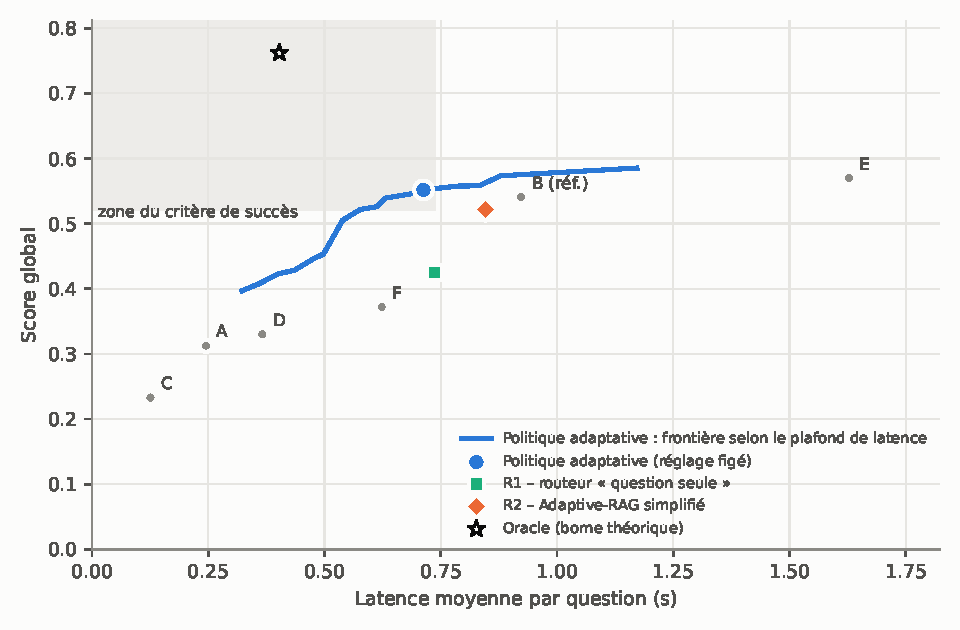
\includegraphics[width=0.78\linewidth]{figures/partie4_qualite_cout.pdf}
\caption{Compromis qualité--latence sur le développement. La courbe bleue donne, pour chaque plafond de
latence, le meilleur score atteignable par la politique ; le point bleu est le réglage figé. La zone
grisée correspond au critère de succès.}
\label{fig:dev}
\end{figure}

Sur le développement, la politique remplit le critère principal (+1,1 point, $-23$~\% de latence) et
dépasse R1 et R2. Deux signaux d'alerte étaient toutefois visibles : la validation croisée estimait une
perte de 2,1 points, à la limite du critère, et les questions simples perdaient 14 points (le critère
de robustesse n'était donc déjà pas satisfait), en échange d'un gain de 21,7 points sur les questions
non couvertes.

%======================================================================
\section{Évaluation finale sur le jeu de test}\label{sec:final}
%======================================================================

\subsection{Exécution}

Les six stratégies fixes et la politique ont été exécutées sur les 450 questions du test, en
\textbf{trois passes complètes}, avec un ordre des méthodes tiré au hasard dans chaque passe pour
répartir l'effet de l'échauffement de la machine. La latence retenue est la médiane des trois passes
pour chaque question. La politique est exécutée réellement de bout en bout. R1 et R2, entraînés sur tout
le développement, sont appliqués aux sorties du test. L'énergie a été mesurée pendant toute
l'évaluation (30\,630 relevés ; puissance au repos 2,7~W).

Deux contrôles valident l'exécution : les réponses sont \textbf{identiques dans les trois passes} pour
toutes les méthodes, et la politique exécutée \textbf{reproduit exactement sa simulation} (accord de
100~\% sur le score, latence à 0,001~s près).

\subsection{Résultats principaux}

\begin{table}[H]
\centering\small\setlength{\tabcolsep}{4pt}
\begin{tabular}{l c c c c c c c}
\toprule
Méthode & Score & IC 95~\% & Écart à B & Latence & P95 & Couv. & Risque \\
\midrule
A -- grand, sans RAG & 0,310 & [0,269 ; 0,351] & $-22{,}7$ & 0,27~s & 0,52~s & 0,45 & 0,76 \\
\textbf{B -- grand, 3 passages (réf.)} & \textbf{0,537} & [0,494 ; 0,581] & -- & \textbf{0,87~s} & 1,26~s & 0,73 & 0,42 \\
C -- petit, sans RAG & 0,223 & [0,187 ; 0,261] & $-31{,}4$ & 0,13~s & 0,25~s & 0,51 & 0,93 \\
D -- petit, 3 passages & 0,414 & [0,372 ; 0,457] & $-12{,}3$ & 0,35~s & 0,53~s & 0,88 & 0,57 \\
E -- grand, 6 passages & 0,567 & [0,523 ; 0,610] & $+3{,}0$ & 1,57~s & 2,23~s & 0,75 & 0,40 \\
F -- petit, 6 passages & 0,398 & [0,357 ; 0,440] & $-13{,}9$ & 0,61~s & 0,87~s & 0,94 & 0,60 \\
\midrule
R1 -- question seule & 0,489 & [0,445 ; 0,534] & $-4{,}7$ & 0,74~s & 1,61~s & 0,68 & 0,48 \\
R2 -- Adaptive-RAG simplifié & 0,517 & [0,473 ; 0,561] & $-2{,}0$ & 0,82~s & 1,39~s & 0,68 & 0,44 \\
\textbf{Politique adaptative} & \textbf{0,550} & [0,505 ; 0,594] & $\mathbf{+1{,}3}$ & \textbf{0,79~s} & 1,38~s & 0,64 & \textbf{0,40} \\
\midrule
\textit{Oracle} & \textit{0,797} & [0,762 ; 0,831] & $+26{,}0$ & \textit{0,36~s} & 1,09~s & 0,64 & 0,18 \\
\bottomrule
\end{tabular}
\caption{Résultats sur le jeu de test (450 questions). Latence : moyenne par question de la médiane des
trois passes.}
\label{tab:resultats}
\end{table}

\begin{figure}[H]
\centering
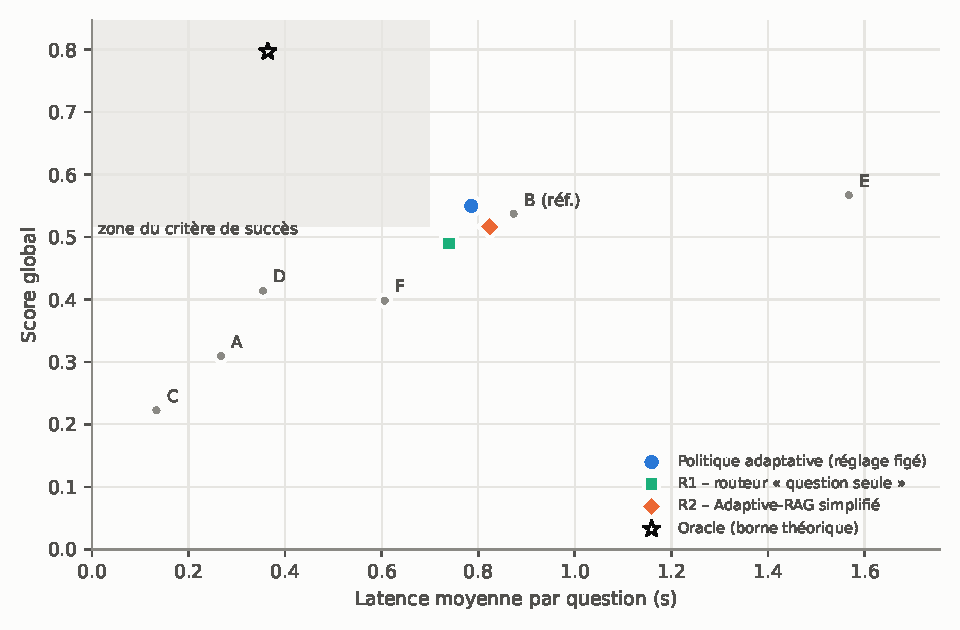
\includegraphics[width=0.78\linewidth]{figures/partie5_qualite_cout.pdf}
\caption{Compromis qualité--latence sur le test. La politique (en bleu) est au-dessus de B, mais à
droite de la zone du critère de succès.}
\label{fig:test}
\end{figure}

\subsection{Verdict sur les critères pré-enregistrés}

\begin{table}[H]
\centering\small
\begin{tabularx}{\linewidth}{Y >{\centering\arraybackslash}p{5.6cm} c}
\toprule
Critère & Mesure & Atteint \\
\midrule
Latence moyenne réduite d'au moins 20~\% & $-10{,}1$~\% (0,786 contre 0,873~s) & \non \\
Perte de score $\le 2$~points & $-1{,}3$ (gain) & \oui \\
Non-infériorité (borne haute de l'IC de la perte $< 2$) & $[-4{,}1\,;\,+1{,}6]$ & \oui \\
\textbf{Critère principal} & & \non \\
\midrule
Risque inférieur à B & 0,395 contre 0,421 & \oui \\
Meilleur score que R1 et R2 & 0,550 contre 0,489 et 0,517 & \oui \\
Aucune catégorie ne perd plus de 5~points & simple $-7{,}6$ ; complexe $-3{,}3$ ; non couverte $+14{,}7$ & \non \\
\bottomrule
\end{tabularx}
\caption{Verdict sur le jeu de test.}
\label{tab:verdict}
\end{table}

L'hypothèse principale est \textbf{rejetée dans sa forme pré-enregistrée} : la politique conserve la
qualité de B avec moins d'erreurs, mais n'économise que la moitié de la latence visée.

\subsection{Par catégorie et choix de la politique}

\begin{table}[H]
\centering\small
\begin{tabular}{l c c c}
\toprule
Méthode & Simple & Complexe & Non couverte \\
\midrule
B -- référence & 0,737 & 0,468 & 0,407 \\
E -- grand, 6 passages & 0,730 & 0,537 & 0,433 \\
R1 & 0,562 & 0,453 & 0,453 \\
R2 & 0,635 & 0,455 & 0,460 \\
\textbf{Politique adaptative} & 0,661 ($-7{,}6$) & 0,435 ($-3{,}3$) & \textbf{0,553} ($+14{,}7$) \\
\textit{Oracle} & 0,842 & 0,682 & 0,867 \\
\bottomrule
\end{tabular}
\caption{Score par catégorie sur le test (150 questions chacune). Entre parenthèses : écart à B.}
\label{tab:categories}
\end{table}

Sur 450 questions, la politique a déclenché 66 abstentions précoces (15~\%) et a fait répondre le grand
modèle 359 fois avec 3 passages et 25 fois avec 6 ; 98 de ces réponses ont ensuite été remplacées par
une abstention finale. L'abstention précoce touche surtout les questions non couvertes (36 sur 150), mais
aussi 18 questions simples et 12 complexes, d'où les pertes sur ces catégories.

\subsection{Ablations}

\begin{table}[H]
\centering\small
\begin{tabular}{l c c c c}
\toprule
& \multicolumn{2}{c}{\textbf{Test}} & \multicolumn{2}{c}{\textbf{Développement}} \\
\textbf{Variante} (chacune réglée sur le développement) & Score & Latence & Score & Latence \\
\midrule
\textbf{Politique complète} & \textbf{0,550} & 0,79~s & 0,552 & 0,71~s \\
Sans recherche adaptative (toujours 3 passages) & 0,547 & 0,74~s & 0,548 & 0,68~s \\
Sans abstention finale & 0,547 & 0,79~s & 0,546 & 0,71~s \\
Sans abstention précoce (cascade petit $\to$ grand) & 0,464 & 0,64~s & 0,395 & 0,70~s \\
Sans aucune abstention & 0,457 & 0,64~s & 0,389 & 0,70~s \\
\bottomrule
\end{tabular}
\caption{Ablations.}
\label{tab:ablations}
\end{table}

L'abstention précoce fondée sur la preuve est la composante décisive ($-8{,}6$~points sans elle sur le
test). La recherche adaptative et l'abstention finale n'apportent chacune que 0,3~point, dans le bruit
statistique ; toujours utiliser 3 passages serait même plus rapide ($-15$~\%) pour un score équivalent.

\subsection{Énergie}

\begin{table}[H]
\centering\small
\begin{tabular}{l c c c}
\toprule
Méthode & Énergie / question & Écart à B & Puissance moyenne \\
\midrule
C -- petit, sans RAG & 1,8~J & $-90$~\% & 16,4~W \\
A -- grand, sans RAG & 3,9~J & $-80$~\% & 17,0~W \\
D -- petit, 3 passages & 7,3~J & $-62$~\% & 23,2~W \\
F -- petit, 6 passages & 13,5~J & $-30$~\% & 24,9~W \\
\textbf{Politique adaptative} & \textbf{17,5~J} & $\mathbf{-9}$~\% & 24,8~W \\
B -- grand, 3 passages (réf.) & 19,3~J & -- & 24,7~W \\
E -- grand, 6 passages & 37,7~J & $+95$~\% & 26,4~W \\
\bottomrule
\end{tabular}
\caption{Énergie de la puce (CPU + GPU + ANE) par question sur le test, moyenne des trois passes.}
\label{tab:energie}
\end{table}

La puissance appelée varie peu (16 à 26~W) : l'énergie suit la durée de calcul, donc le nombre de tokens
traités. L'économie d'énergie de la politique ($-9$~\%) suit sa réduction de latence ($-10$~\%).

\subsection{Du développement au test}

\begin{table}[H]
\centering\small
\begin{tabular}{l c c c c}
\toprule
& \multicolumn{2}{c}{Développement (180)} & \multicolumn{2}{c}{Test (450)} \\
Méthode & Score & Latence & Score & Latence \\
\midrule
B -- référence & 0,541 & 0,92~s & 0,537 & 0,87~s \\
Politique adaptative & 0,552 & 0,71~s ($-23$~\%) & 0,550 & 0,79~s ($-10$~\%) \\
R1 & 0,425 & 0,74~s & 0,489 & 0,74~s \\
R2 & 0,522 & 0,85~s & 0,517 & 0,82~s \\
Oracle & 0,762 & 0,40~s & 0,797 & 0,36~s \\
\midrule
Abstentions précoces & \multicolumn{2}{c}{45 / 180 (25~\%)} & \multicolumn{2}{c}{66 / 450 (15~\%)} \\
\bottomrule
\end{tabular}
\caption{Comparaison entre développement et test.}
\label{tab:dev-test}
\end{table}

\textbf{La qualité s'est généralisée}, mieux même que ne le prévoyait la validation croisée (0,550 au
lieu de 0,520). \textbf{Le gain de latence ne s'est pas généralisé} : le seuil d'abstention précoce,
réglé sur 60 questions par catégorie, coupait 25~\% des questions de développement mais n'en coupe que
15~\% sur le test, un écart d'environ trois erreurs-types, attribuable à la variabilité d'échantillonnage
d'un petit jeu de réglage. Moins d'abstentions précoces signifie plus d'appels au grand modèle, donc une
latence plus proche de celle de B.

%======================================================================
\section{Discussion}\label{sec:discussion}
%======================================================================

\paragraph{Retour sur les hypothèses.}
\begin{description}[style=sameline,leftmargin=1cm]
\item[H1 -- rejetée.] Aucun signal calculé avant génération n'a permis d'orienter des requêtes vers le
petit modèle sans perte : R1 perd 4,7 à 11,6 points, et la politique réglée n'utilise jamais le petit
modèle.
\item[H2 -- non confirmée.] La politique a un risque plus faible que B, mais l'apport de la confiance du
modèle en plus de la preuve est négligeable (0,3 point, risque inchangé). C'est la preuve seule qui
porte le gain.
\item[H3 -- partiellement confirmée.] La politique n'est dominée par aucune stratégie fixe ni aucun
routeur (aucun n'est à la fois meilleur et plus rapide), et elle domine B. Mais son gain de coût est
modeste.
\item[H4 -- confirmée.] Les effets sont très hétérogènes : $-7{,}6$ points sur les questions simples,
$+14{,}7$ sur les questions non couvertes. Une moyenne seule aurait masqué ce compromis.
\end{description}

\paragraph{Enseignements.}
\begin{enumerate}
\item \textbf{La preuve est un meilleur signal de routage que la question.} À latence comparable, la
politique dépasse R1 de 6 points et R2 de 3 points. Regarder ce que la recherche a trouvé renseigne
mieux que deviner la difficulté d'après la formulation, ce qui rejoint \citet{li2026beyond}.
\item \textbf{L'abstention rend l'adaptation rentable.} Ne pas générer sur une preuve faible économise du
calcul et évite des erreurs en même temps.
\item \textbf{Le petit modèle n'a pas trouvé sa place.} Sa confiance ne signale ses erreurs que
modérément (AUC 0,74) et chaque escalade paie deux générations.
\item \textbf{La marge reste considérable.} L'oracle atteint 0,797 en 0,36~s : les bons choix existent,
c'est leur prédiction qui est difficile.
\end{enumerate}

%======================================================================
\section{Points faibles et améliorations}\label{sec:faiblesses}
%======================================================================

Cette section recense les faiblesses de l'étude, de la plus importante à la moins importante, et pour
chacune l'amélioration proposée. Le tableau~\ref{tab:faiblesses} en fait la synthèse.

\subsection{Faiblesses de la méthode}

\paragraph{F1 -- Seuils absolus réglés sur un petit échantillon.} C'est la cause directe de l'échec du
critère principal. Un seuil sur une valeur absolue de la preuve, réglé sur 60 questions par catégorie,
ne déclenche pas la même proportion d'abstentions sur une autre distribution de questions. La
validation croisée, faite sur le même petit échantillon, ne pouvait pas le révéler.
\emph{Améliorations :} (i) exprimer les seuils comme des \emph{quantiles} ou un \emph{budget} (« s'abstenir
sur les $x$~\% de questions aux preuves les plus faibles »), ce qui garantit le taux d'abstention, donc
la latence ; (ii) calibrer les seuils avec une méthode conforme, qui donne des garanties de risque sans
hypothèse sur la distribution \citep{hao2026racer} ; (iii) agrandir le jeu de réglage à au moins
500 questions ; (iv) régler avec une marge de sécurité dérivée de la variabilité observée par bootstrap,
et non fixe.

\paragraph{F2 -- Perte sur les questions simples ($-7{,}6$~points).} L'abstention précoce touche aussi
18 questions simples et 12 complexes sur 150 : un score BM25 faible ne signifie pas toujours que la
réponse est absente (reformulation, synonymes). La couverture baisse de 0,73 à 0,64.
\emph{Améliorations :} (i) remplacer la preuve lexicale par un juge de suffisance léger (re-classeur
\emph{cross-encoder} ou petit modèle d'inférence, dans l'esprit de CRAG \citep{yan2024crag} et
Tiny-Critic RAG \citep{wu2026tinycritic}) ; (ii) combiner preuve BM25 et preuve dense ; (iii) ajouter au
réglage une contrainte par catégorie, de sorte qu'aucune ne perde plus de 5~points.

\paragraph{F3 -- Signaux de confiance faibles.} Aucun signal ne dépasse une AUC de 0,74, et l'abstention
finale n'apporte que 0,3~point. La probabilité des tokens d'une réponse courte informe mal sur sa
justesse. \emph{Améliorations :} entropie sémantique \citep{kuhn2023semantic} ou cohérence entre
quelques échantillons, réservées aux cas limites pour en contenir le coût ; sonde entraînée sur les
états internes du modèle \citep{kadavath2022know}.

\paragraph{F4 -- Recherche adaptative quasi inutile.} Choisir 6 passages au lieu de 3 ne concerne que
6~\% des questions et n'apporte rien de mesurable. Or les questions complexes ont un rappel@3 de
seulement 0,37 : le problème n'est pas le \emph{nombre} de passages mais la recherche elle-même.
\emph{Améliorations :} décomposition ou reformulation des questions multi-étapes, recherche itérative
déclenchée par l'incertitude \citep{jiang2023flare,su2024dragin}, compression du contexte pour réduire
le coût des passages supplémentaires \citep{arefeen2024leancontext}.

\paragraph{F5 -- Le petit modèle est inutilisé.} La politique finale n'utilise qu'un seul modèle : la
dimension « choix du modèle » de la question de recherche n'est pas réellement exploitée.
\emph{Améliorations :} essayer un petit modèle plus performant ou spécialisé en extraction, ou l'employer
pour un rôle moins exigeant (vérification, reformulation de requête) ; décodage spéculatif, où le petit
modèle accélère le grand sans changer ses réponses.

\paragraph{F6 -- Latence de queue dégradée.} La latence P95 de la politique (1,38~s) dépasse celle de B
(1,26~s) à cause des réponses à 6 passages. \emph{Amélioration :} inclure le P95 dans l'objectif de
réglage, ou plafonner le contexte.

\paragraph{F7 -- Écart à l'oracle de 25~points.} \emph{Amélioration :} un routeur appris combinant
caractéristiques de la question, preuve et confiance, entraîné sur un jeu bien plus grand que
180 questions.

\subsection{Faiblesses du protocole}

\paragraph{F8 -- Benchmark construit et restreint.} Questions en anglais tirées de SQuAD 2.0 et
HotpotQA, corpus fermé de 3\,293 passages ; les questions non couvertes sont des questions adverses de
SQuAD 2.0, rédigées pour ressembler aux passages, ce qui n'est pas représentatif de l'usage réel ; la
catégorie des questions ambiguës, prévue au protocole, n'a pas été annotée.
\emph{Améliorations :} ajouter MuSiQue \citep{trivedi2022musique} et CRAG \citep{yang2024cragbench},
un corpus réel en français, et annoter au moins 50 questions ambiguës.

\paragraph{F9 -- Métrique lexicale.} Le F1 pénalise les réponses correctes formulées autrement
(paraphrase, synonyme, date écrite autrement). \emph{Amélioration :} juge sémantique (modèle d'inférence
ou LLM juge), validé sur un échantillon annoté à la main.

\paragraph{F10 -- Puissance statistique limitée.} Avec 450 questions, l'intervalle de confiance du score
est large d'environ $\pm 4{,}4$~points : un écart de 2~points, le seuil du critère, n'est pas
détectable avec certitude. \emph{Amélioration :} jeu de test d'au moins 1\,500 questions.

\paragraph{F11 -- Matériel et mesure uniques.} Un seul appareil (M3 Pro, MLX, 4 bits) ; l'énergie est
celle de la puce, pas la consommation murale. \emph{Améliorations :} répliquer sur GPU NVIDIA et avec
\texttt{llama.cpp}, mesurer au wattmètre, rapporter la mémoire.

\paragraph{F12 -- Conception explorée sur le développement.} Deux conceptions ont été essayées avant de
figer la politique ; c'est documenté, mais cela augmente le risque de sur-ajustement au développement.
\emph{Amélioration :} pré-enregistrer aussi la \emph{famille} de politiques, et pas seulement les
critères. Toute amélioration devra être évaluée sur un \textbf{nouveau} jeu de test : celui-ci est
désormais consommé.

\paragraph{F13 -- Revue de littérature à approfondir.} L'état de l'art a d'abord été établi à partir
des résumés des articles. \emph{Amélioration :} lecture complète des travaux les plus proches
(Adaptive-RAG, \citealp{moskvoretskii2025adaptive}, RAGRouter-Bench, RACER, \citealp{li2026beyond})
pour confirmer le positionnement du tableau~\ref{tab:positionnement}.

\begin{table}[H]
\centering\small
\begin{tabularx}{\linewidth}{c Y Y c}
\toprule
& Faiblesse & Amélioration principale & Priorité \\
\midrule
F1 & Seuils absolus, petit jeu de réglage & Seuils en quantiles / budget, calibration conforme, $\ge 500$ questions & Haute \\
F2 & Perte sur les questions simples & Juge de suffisance léger, contrainte par catégorie & Haute \\
F10 & Puissance statistique & Test $\ge 1\,500$ questions & Haute \\
F3 & Signaux de confiance faibles & Cohérence entre échantillons sur les cas limites & Moyenne \\
F4 & Recherche adaptative inutile & Décomposition des questions multi-étapes & Moyenne \\
F8 & Benchmark restreint & MuSiQue, CRAG, corpus français, questions ambiguës & Moyenne \\
F9 & Métrique lexicale & Juge sémantique validé & Moyenne \\
F5 & Petit modèle inutilisé & Autre petit modèle, décodage spéculatif & Moyenne \\
F13 & Revue fondée sur les résumés & Lecture complète des travaux proches & Moyenne \\
F6 & Latence P95 & P95 dans l'objectif de réglage & Basse \\
F7 & Écart à l'oracle & Routeur appris multi-signaux & Basse \\
F11 & Matériel unique & Réplication GPU, wattmètre & Basse \\
F12 & Exploration sur le développement & Pré-enregistrer la famille de politiques & Basse \\
\bottomrule
\end{tabularx}
\caption{Synthèse des points faibles et des améliorations.}
\label{tab:faiblesses}
\end{table}

%======================================================================
\section{Conclusion}\label{sec:conclusion}
%======================================================================

Nous avons construit un benchmark et un protocole pré-enregistrés pour évaluer, sur une machine
personnelle, l'allocation adaptative du calcul et de la recherche documentaire. Après avoir montré que
les routeurs fondés sur la question seule ne suffisent pas, nous avons proposé une politique qui décide
conjointement du modèle, du nombre de passages et de l'abstention à partir de la preuve BM25 et de la
confiance du modèle. Sur le jeu de test, elle préserve la qualité de la configuration de référence, fait
moins d'erreurs et dépasse les deux routeurs de référence ; mais elle ne réduit la latence que de 10~\%
et l'énergie de 9~\%, au lieu des 20~\% visés. L'hypothèse principale est donc rejetée dans sa forme
pré-enregistrée.

Deux enseignements dépassent ce résultat : sur machine locale, \emph{la qualité des preuves récupérées
est un signal de routage plus utile que la question elle-même}, et \emph{savoir s'abstenir est ce qui
permet d'économiser sans dégrader la fiabilité}. La prochaine étape est de rendre ce levier stable :
exprimer l'abstention comme un budget calibré plutôt qu'un seuil absolu, mieux juger la suffisance des
preuves, et valider le tout sur un jeu de test plus grand et neuf.

\paragraph{Reproductibilité.} Code, benchmark (avec empreintes des données), configurations figées
(étiquettes \texttt{protocole-v1.0} et \texttt{politique-v1.0}), sorties brutes des trois passes et
mesures d'énergie sont publiés dans le dépôt indiqué en première page.

\bibliographystyle{plainnat}
\bibliography{references}

\appendix
\section{Prompts}\label{ann:prompts}
\textbf{Sans recherche documentaire :}
\begin{small}
\begin{verbatim}
Answer the question with a short phrase only. If you do not know the answer
or it cannot be determined, reply exactly: UNANSWERABLE.

Question: {question}
Answer:
\end{verbatim}
\end{small}
\textbf{Avec recherche documentaire :}
\begin{small}
\begin{verbatim}
Answer the question using only the passages below, with a short phrase only.
If the passages do not contain the answer, reply exactly: UNANSWERABLE.

[1] {titre}: {texte}
[2] ...

Question: {question}
Answer:
\end{verbatim}
\end{small}

\end{document}
